\newpage

\section{Proposed Method}
\label{sec:04_method}

\subsection{Architecture}
\begin{figure}[htbp]
    \centering
    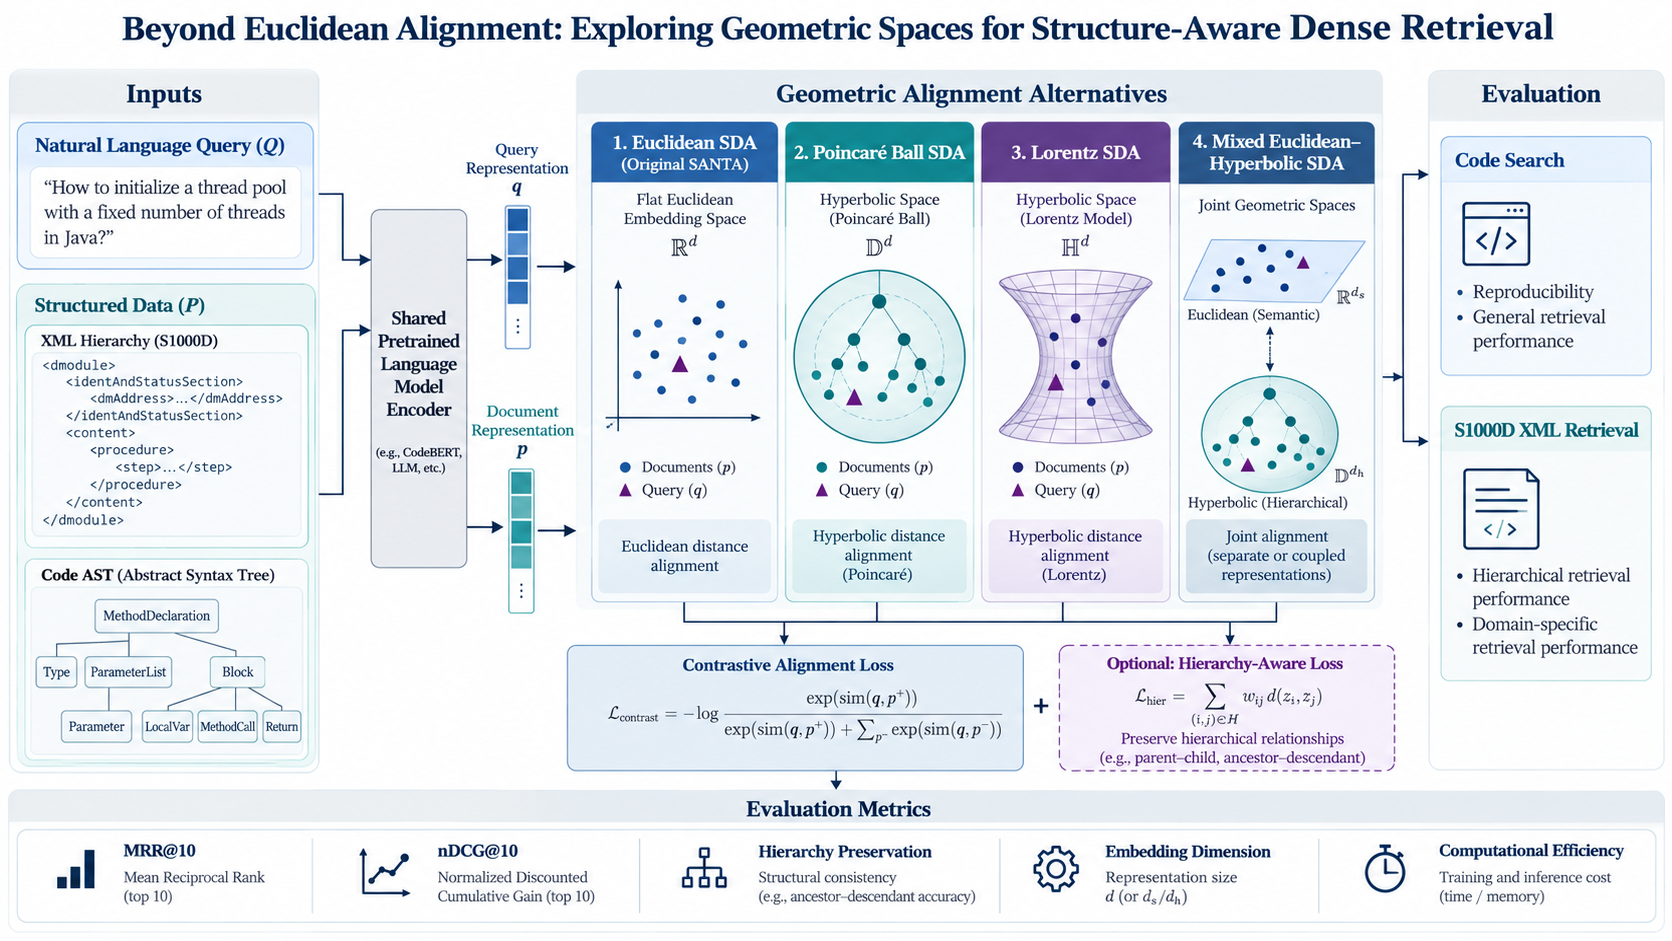
\includegraphics[width=\textwidth]{images/overview_ai.png}
    \caption{Conceptual architecture of geometric alignment for structure-aware dense retrieval. The diagram summarizes candidate alignment geometries and evaluation settings; the mixed-geometry branch and hierarchy-aware objective represent optional extensions.}
    \label{fig:architecture}
\end{figure}
% Refine the architecture description once the alignment variants are finalized.

\subsection{Structure-Aware Representations}
% Describe how semantic and structural information enter the representations.

\subsection{Geometric Alignment}
% Define the alignment mechanism and its mathematical assumptions.

\subsection{Learning Objectives and Optimization}
% Specify losses, supervision, optimization, and safeguards against information leakage.

\subsection{Retrieval Procedure}
% Describe query encoding, document indexing, scoring, and ranking at inference.

